\sectionquestion{TA Questions (DO NOT TEST THIS SECTION)}

This section is for TAs to put their draft questions into. Please see the qtemplates.tex file for how to format the questions. 

\begin{parts}

\part[5] [Sana, Weyxin] You are performing a linear regression on a dataset that consists of $2m$ points and $m$ features. Your friend, Lucy, suggests using a closed-form solution to obtain your parameter estimates, $\hat{\theta}$. Another friend, Josh, suggests that stochastic gradient descent is a better approach. They get into a heated debate and turn to you to resolve it. 

\begin{subparts}
    
    \subpart[2] What is the computational complexity for the closed-form solution in terms of $m$? Recall that the closed form solution is $(X^TX)^{-1}X^T Y$.
    
    \begin{soln}
     The closed form solution is $(X^TX)^{-1}X^T Y$ for $X \in \mathbb{R}^{n \times m}$ and $Y \in \mathbb{R}^{n \times 1}$\\[0.1 in]
     $X^TX$: $O(m^2 n)$\\[0.05 in]
     $(X^T X)^{-1}: O(m^3)$\\[0.05 in]
     $X^T Y: O(mn)$\\[0.05 in]
     $(X^T X)^{-1} (X^T Y): O(m^2)$\\[0.1 in]
     The computational complexity for the closed form solution is:\\[0.05 in]
     $O(m^2 n) + O(m^3) + O(mn) + O(m^2)$\\[0.05 in]
     $\in O(m^2 n) + O(m^3)$ \\[0.05 in]
     $= O(2m^3) + O(m^3) \hspace{0.2 in}$ since $n=2m$\\[0.05 in]
     $\in \boxed{O(m^3)}$
    \end{soln}
    
    \subpart[2] What is the computation complexity for one pass of stochastic gradient descent in terms of $m$?

    
    \begin{soln}
     The computational complexity for SGD is:\\[0.05 in]
     $O(mn) \hspace{0.37 in}$ since we only perform 1 iteration\\[0.05 in]
     $= O(2m^2) \hspace{0.2 in}$ since $n=2m$\\[0.05 in]
     $\in \boxed{O(m^2)}$
    \end{soln}
    
    \subpart[1] Assuming a closed-form solution is attainable and only one pass of stochastic gradient descent is required to obtain convergence to the optimal $\hat{\theta}$, who is correct and why? Justify with the computational complexities of both approaches.
    
    \begin{soln}
     Josh is correct. The computational time for SGD is $O(m^2)$, while the computational time for the closed form solution is $O(m^3)$. Thus, SGD is more computationally efficient.
    \end{soln}
\end{subparts}

\part[8] [Joseph] Consider the following training data. The red "$-$" marks represent $Y=0$ and the blue "$+$" marks represent $Y=1$.

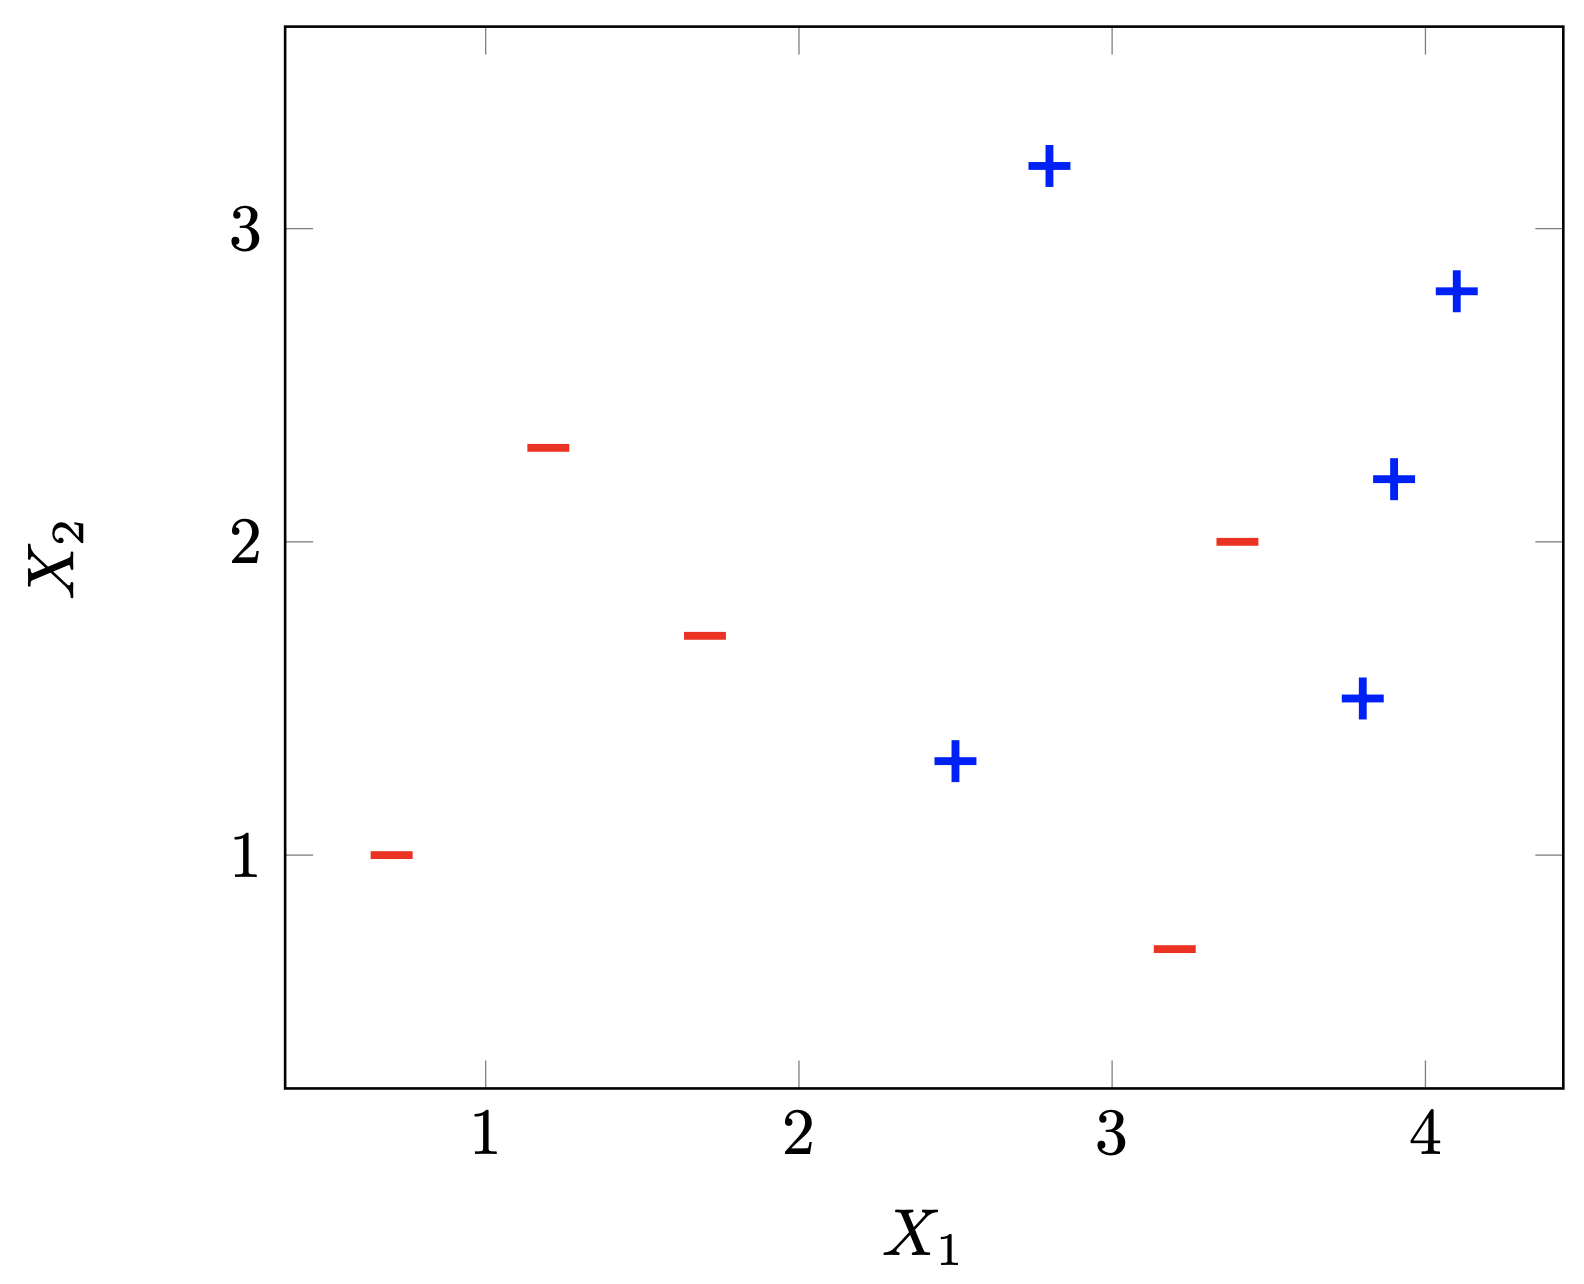
\includegraphics[scale=0.5]{exam1/figures/DecisionTreeData.png}

\begin{subparts} 
    \subpart[2] What is the entropy, $H(Y)$, of the entire dataset? Give your numerical answer in number of bits (i.e. using $\log_2$) with at least two decimal places. (We expect that you are able to compute this numerical value by hand.)
    
    \begin{soln}
     $1 \pm 0.001$
    \end{soln}
    
    \subpart[2] What is the mutual information if we are splitting on $X_2 < 2.5$? Write your answer as an arithmetic expression that includes $\log_2$ operations but doesn't include symbolic information such as $H$.
    
    \begin{soln}
    $1 - (0.2 \cdot 0 + 0.8 \cdot (-5/8 \cdot \log_2 (5/8) - 3/8 \cdot \log_2 (3/8))) = 0.23645$
    \end{soln}
    
    \subpart[2] Using error rate as the splitting criteria, which of the following is the best choice for the first binary split?
    
    \begin{enumerate}[label=\Alph*]
        \item $X_1 < 2$ and $X_1 \ge 2$
        \item $X_1 < 3$ and $X_1 \ge 3$
        \item $X_2 < 2.5$ and $X_2 \ge 2.5$
    \end{enumerate}
    
    \begin{soln}
     $X_1 < 2$ and $X_1 \ge 2$
    \end{soln}
    
    \subpart[1] If the tree only has one binary split (i.e. a decision stump), what would be the lowest training error rate we can get?
    
    \begin{soln}
    $0.2 \pm 0.001$
    \end{soln}
    
    \subpart[1] True or false: It is possible to have a decision tree with zero training error for this dataset. Assume only binary splits and attributes selected with replacement.
    
    \begin{enumerate}[label=\Alph*]
        \item True
        \item False
    \end{enumerate}
    
    \begin{soln}
    True
    \end{soln}
\end{subparts}

\part[4] [Helena] MOVED

\newpage

\part[8] [Chi Gao] Consider the following data set of (x, y):

\begin{figure}[h]
    \centering
    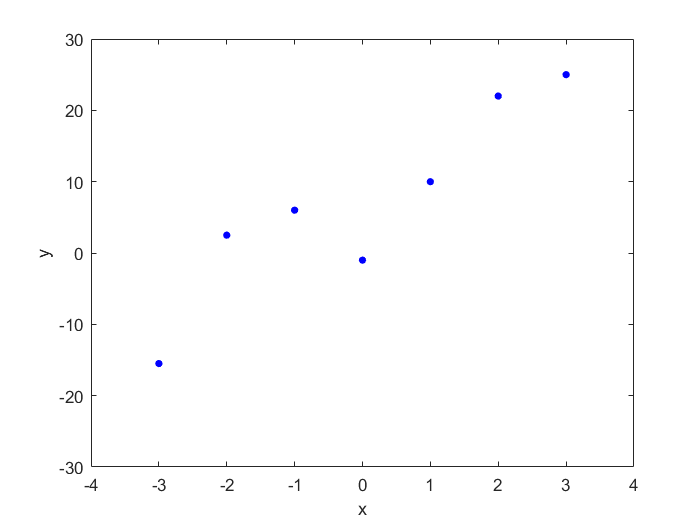
\includegraphics[scale=0.5]{exam1/figures/regularization_question.png}
\end{figure}

After some feature engineering work, your friend Pac built a linear regression model:

\begin{align*}
    y = \theta^T\mathbf{x} + b
    \text{  where  }
    \theta = \begin{bmatrix}
        -0.5 \\
        0.5 \\
        5 \\
        2.5
    \end{bmatrix}
    \text{ , }
    \mathbf{x} = \begin{bmatrix}
        x^4 \\
        x^3 \\
        x^2 \\
        x
    \end{bmatrix}
    \text{  and  }
    b = 1.5
\end{align*}

\begin{figure}[h]
    \centering
    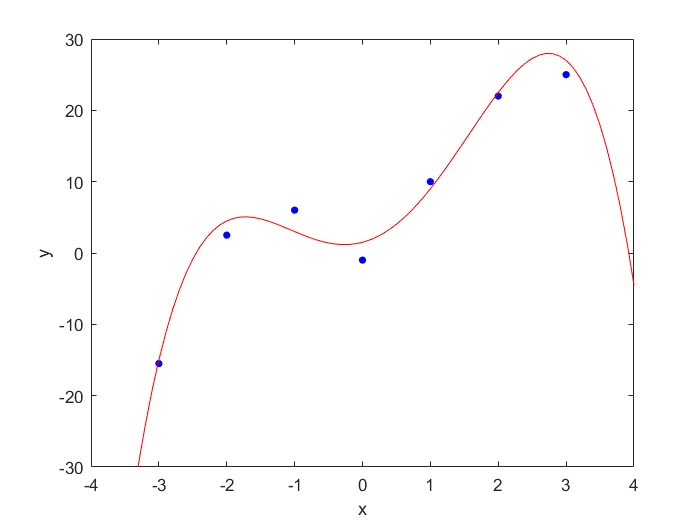
\includegraphics[scale=0.5]{exam1/figures/regularization_model.png}
\end{figure}

\begin{subparts} 
    \subpart[2] Pac's model results in poor accuracy during the validation data test. What is the potential problem in his feature engineering? 
    
    \begin{soln}
     Pac created too many extra features and his model is overfitting.
    \end{soln}
    
    \subpart[3] Based on the problem pointed out in the previous part, which type of the following regularization terms would you introduce to Pac's model to improve it? Justify your choice and calculate the value of the term you choose. 
    
    \begin{list}{}
     \item\Circle{} L1 regularization
     \item\Circle{} L2 regularization
    \end{list}
    
    \begin{soln}
    Use L1 regularization, since we want to reduce the weight of unnecessary features to zero. The result is:
    \begin{equation*}
    \sum|\theta_k| = 0.5 + 0.5 + 5 + 2.5 = 8.5
    \end{equation*}
    \end{soln}
    
    \subpart[3] Suppose the $y$ values of all data points are increased by 1.5 and Pac's model is correspondingly shifted. Would your regularization term in the previous part change? If your answer is "Yes", calculate the change in your regularization term. If "No", justify your answer.
    
    \begin{soln}
    No. Because the purpose of regularization is to control the weights of parameters and reduce unnecessary features. We should not penalize the learning algorithm due to the shift of all data points, and including bias term in the regularization defeats this purpose. (p.s. should we consider the case when the bias term is folded? personally I think we should still not penalize it even when it is folded in.)
    \end{soln}
\end{subparts}

% KNN
\part[2] [Mukund] Two statements are given below. Which of the following are true?


\indent{1. The k-NN classifier adapts as we collect new training data.}

\indent{2. The computational complexity for classifying new data points grows linearly with the number of samples in the training data set in the worst-case scenario.}

    \begin{enumerate}[label=\Alph*]
        \item 1
        \item 2
        \item 1 and 2
        \item Neither
    \end{enumerate}
    
    \begin{soln}
    1 and 2
    \end{soln}

\part[3] [Mukund] MOVED

%%%%%%%%%%%%%%%%%%%%%%%%%%%%%%%%%%%%%%%%%%%%%%%%%%%%%%%%%%%%%%%%%%%%%%%
% Logistic Regression 
\part[1] \textbf{Select one:} In logistic regression seen in class, we assume that the likelihood of an example $x^{(i)}$ having a positive label is:
\begin{center}
    \[p(y = 1 | x^{(i)}) = \frac{1}{1 + exp(-\thetav^T x^i)} \]
\end{center}
We also defined a loss function
\begin{center}
    \[J(\thetav) = \frac{1}{N} \sum_{i=1}^N {-log (p(y = 1 | x^{(i)}, \thetav))}\]
\end{center}
We then trained on data to discover the optimal $\thetav$.

What is the correct interpretation of gradient descent in the logistic regression setting during training?
    \begin{checkboxes}
     \choice We are minimizing the loss function with respect to the labels $y$.
     \choice We are maximizing the likelihood of the training data with respect to all examples $x^{(i)}$.
     \choice We are maximizing the loss function with respect to the weights $\thetav$.
     \choice We are maximizing likelihood of the training data with respect to the weights $\thetav$.
    \end{checkboxes}
    \begin{soln}
    We are maximizing likelihood with respect to the weights $\thetav$.
    \end{soln}
    \begin{qauthor}
    Kevin Liu, 
    3a Apply the principle of maximum likelihood estimation (MLE) to learn the parameters
    of a probabilistic model
    \end{qauthor}
    
\part[1] \textbf{Select all that apply:} When working with likelihood functions, we often use the negative log likelihood to define a loss function. Why do we do this?
    {%
    \checkboxchar{$\Box$} % change checkbox style locally
    \begin{checkboxes}
     \choice The negative log function is strictly increasing. We want to maximize the loss by maximizing the negative log loss.
     \choice The negative log function is strictly increasing. We want to minimize the loss by minimizing the negative log loss.
     \choice The log function makes some likelihood functions easier to rearrange into an update rule by simplifying exponents and multiplication.
     \choice The negative log function is strictly decreasing. We want to minimize the loss by minimizing the negative log loss.
    \end{checkboxes}
    }
    \begin{soln}
     The negative log function is strictly decreasing. We want to minimize the loss by minimizing the negative log loss.
     The log function makes some likelihood functions easier to simplifying exponents and multiplication.
    \end{soln}
    \begin{qauthor}
    Kevin Liu, 
    3c. Explain the practical reasons why we work with the log of the likelihood
    \end{qauthor}
    
\part[20] In class, we applied Maximum Likelihood Estimation to derive an update rule for binary logistic regression. The same process can be used to find parameters for other probabilistic models. In this question, we will apply MLE to a Gaussian clustering problem.

We have a set of data points $x^{(i)} \in \mathbb{R}$ that we know is independently, identically distributed in the same normal distribution. We want to learn the parameters of the true distribution $\mu, \sigma$. To do so, we will use stochastic gradient descent. (In reality, in batch learning, there is a closed form solution to single Gaussian clustering. For the sake of this problem, we will use SGD instead.)

The probability of a data point belonging to the distribution is:
\begin{center}
    \[p(y = 1 | x) = \frac{1}{2 \pi} e^{-\frac{1}{2}(\frac{x-\mu}{\sigma})^2}\]
\end{center}
Note: In this problem, a label of 1 means that the point belongs to our distribution. We are assuming that all our data points belong to this same Gaussian distribution. In short, don't worry about $p(y=0 | x)$!
    \noaddpoints % to omit double points count
    \begin{subparts}
    \subpart[10] \textbf{Short answer:} Using the process shown in class, derive an expression for the gradient $\frac{d J(\mu, \sigma)}{d \mu}$ for the SGD update step for the mean, where $J(\thetav)$ is the negative log likelihood of the data. $\sigma, \mu$ are yet unknown, so leave them in the expression.
    \fillwithlines{2em}
    \begin{soln}
    \[p(y = 1 | x, \mu, \sigma) = \frac{1}{2 \pi} e^{-\frac{1}{2}(\frac{x-\mu}{\sigma})^2}\]
    \[\ell(x | \mu, \sigma) = log[\frac{1}{2 \pi} e^{-\frac{1}{2}(\frac{x-\mu}{\sigma})^2}]\]
    \[ = log(\frac{1}{2 \pi}) + (-\frac{1}{2}(\frac{x-\mu}{\sigma})^2)\]
    \[-\ell(x | \mu, \sigma) = -log(\frac{1}{2 \pi}) + \frac{1}{2}(\frac{x-\mu}{\sigma})^2 = J(\mu, \sigma)\]
    \[\frac{d J(\mu, \sigma)}{d \mu} = \frac{\mu - x}{\sigma^2}\]
    \end{soln}
    \begin{qauthor}
    Kevin Liu,
    a. Apply the principle of maximum likelihood estimation (MLE) to learn the parameters
    of a probabilistic model
    b. Given a discriminative probabilistic model, derive the conditional log-likelihood, its
    gradient, and the corresponding Bayes Classifier
    \end{qauthor} 
    \subpart[10] \textbf{Numerical answer:} With gradient in hand, you begin training your Gaussian model. You initialize your parameters like so: $\mu = 3, \sigma = 2$. The first point you encounter is $x^{(1)} = 6$. Assume a learning rate of 0.1. What is the new value of $\mu$?
    \begin{tcolorbox}[fit,height=1cm, width=2cm, blank, borderline={1pt}{-2pt}]
    %solution
    \end{tcolorbox}
    \begin{soln}
    Based on the gradient solved from the previous part, we have that
    \[\frac{d J(\mu, \sigma)}{d \mu} = \frac{\mu - x}{\sigma^2} = \frac{3 - 6}{2 ^2} = \frac{-3}{4}\]
    We do one update step with SGD on this single example.
    \[\mu' = \mu - \alpha * \frac{d J(\mu, \sigma)}{d \mu} = 3 - 0.1 * -0.75 = 3.075 \]
    Therefore, our answer is 3.075.
    \end{soln}
    \begin{qauthor}
    Input (1) author name, (2) learning objective addressed, and (3) source if  adapting/reusing a question.
    \end{qauthor}
    \end{subparts}
    \addpoints
    

%%%%%%%%%%%%%%%%%%%%%%%%%%%%%%%%%%%%%%%%%%%%%%%%%%%%%%%%%%%%%%%%%%%%%%
% Overview / Decision Trees

\part[1] MOVED

\part[3] MOVED

\part[2] MOVED
    
\part[2] [Sami] 
Consider the two following multilayer perceptrons.
    \begin{figure}[h]
    \centering
    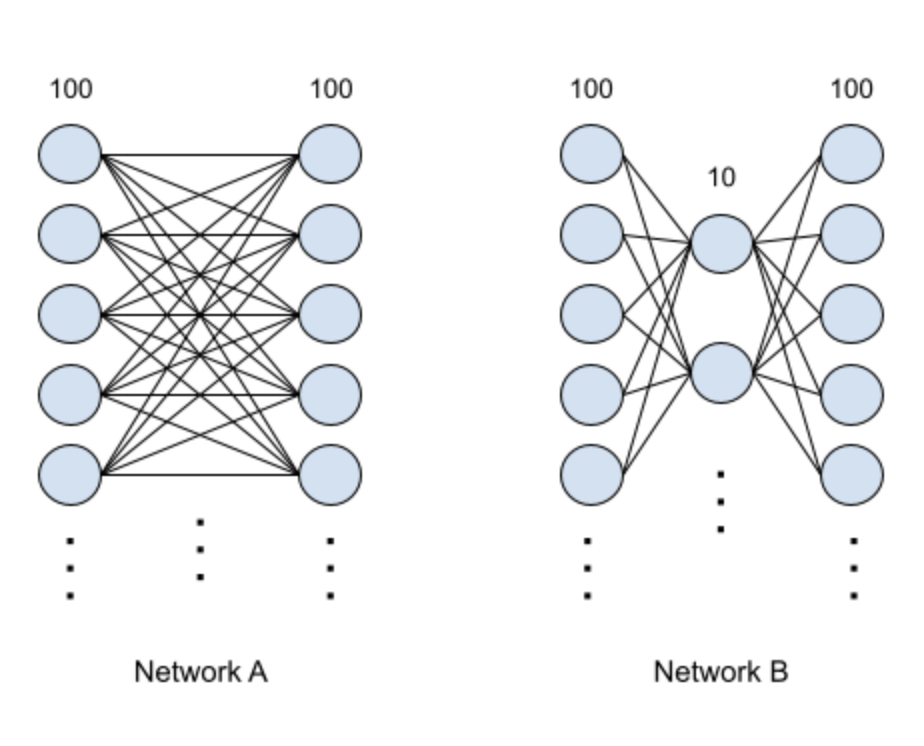
\includegraphics[scale=0.5]{exam1/figures/perceptron_network.png}
    \end{figure}
    \noaddpoints % to omit double points count
    \begin{subparts}
    \subpart[1] \textbf{Short answer:} 
    Describe one advantage of Network A over Network B.
    \fillwithlines{2em}
    \begin{soln}
    A is more expressive than B.
    \end{soln}
    \begin{qauthor}
    Abhishek Vijayakumar, 1.a
    \end{qauthor}
    
    \subpart[1] \textbf{Short answer:} Describe one advantage of Network B over Network A. 
    \fillwithlines{2em}
    \begin{soln}
    B has fewer connections, so it is less prone to overfitting.
    \end{soln}
    \begin{qauthor}
    Samiksha Kale, .
    \end{qauthor}
    
    \end{subparts}

\part[2] [Sami] Suppose you initialize a Perceptron with parameters $\wv = [-3, 1]^T$ and $b = -2$. Then, you start training the perceptron and the first example that comes through has features $\xv = [1, 2]^T$ and label $y = +1$.

\begin{subparts}

    \subpart[1] How is this new point classifed by the Perceptron?
    \begin{checkboxes}
     \choice $\hat{y} = +1$
     \choice $\hat{y} = -1$
    \end{checkboxes}
    \begin{soln}
    $\hat{y} = -1$
    \end{soln}
    \begin{qauthor}    Sami    \end{qauthor}
    
    
    \subpart[1] What are the parameters $\wv$ and $b$ after one iteration of the perceptron training algorithm?
    \begin{tcolorbox}[fit,height=1cm, width=2cm, blank, borderline={1pt}{-2pt}]
    %solution
    \end{tcolorbox}
    \begin{soln}
    $\wv = [-2, 2]$ and $b = -1$
    \end{soln}
    \begin{qauthor}    Sami    \end{qauthor}

\end{subparts}


\part[2] [Sami] Suppose you keep training the same perceptron. The next training example arrives with features $\xv = [1, 2]^T$ and label $y = +1$. 

\begin{subparts}

    \subpart[1] How is this new point classifed by the Perceptron?
    \begin{checkboxes}
     \choice $\hat{y} = +1$
     \choice $\hat{y} = -1$
    \end{checkboxes}
    \begin{soln}
    $\hat{y} = +1$
    \end{soln}
    \begin{qauthor}    Sami    \end{qauthor}
    
    
    \subpart[1] What are the parameters $\wv$ and $b$ after one iteration of the perceptron training algorithm?
    \begin{tcolorbox}[fit,height=1cm, width=2cm, blank, borderline={1pt}{-2pt}]
    %solution
    \end{tcolorbox}
    \begin{soln}
      nothing changes $\wv = [-2, 2]$ and $b = -1$
    \end{soln}
    \begin{qauthor}    Sami    \end{qauthor}

\end{subparts}

\part MOVED

'\part[3] \textbf{Short answer:} Suppose you'd like to fit a decision tree classifier for a classification problem. You're (rightly) concerned about overfitting, so you decide to use two methods to prevent it: a maximum depth and a mutual information threshold. Briefly describe an algorithm for choosing optimal values for these two hyperparameters using grid search.

% provide vignette for context - allow students to interpret

    \fillwithlines{2em}
    \begin{soln}
    Split data into train, test, validation. Choose an appropriate set of values for both max depth and MI threshold and loop through all possible pairs of these values. For each pair, train a decision tree using the specific hyperparameter values and calculate validation error. Choose the pair with lowest validation error. 
    \end{soln}
    \begin{qauthor}
    Brendon
    \end{qauthor}
    
\part[3] MOVED
%%%%%%%%%%%%%%%%%%%%%%%%%%%%%%%%%%%%%%%%%%%%%%%%%%%%%%%%%%%%%%%%%%%%%%

\end{parts}